\documentclass{article}
\usepackage[utf8]{inputenc}
\usepackage{graphicx}
\usepackage[top=2cm, bottom=2cm, left=2cm, right=2cm]{geometry}

\title{INFO-F-303 Base de données\\ Projet : Annuaire d’établissements horeca \\ Rapport de première partie}
\author{Hakim Boulahya \& Youcef Bouharaoua}
\date{April 2016}

\begin{document}

\maketitle

\section*{Modèle entité-association}


\centerline{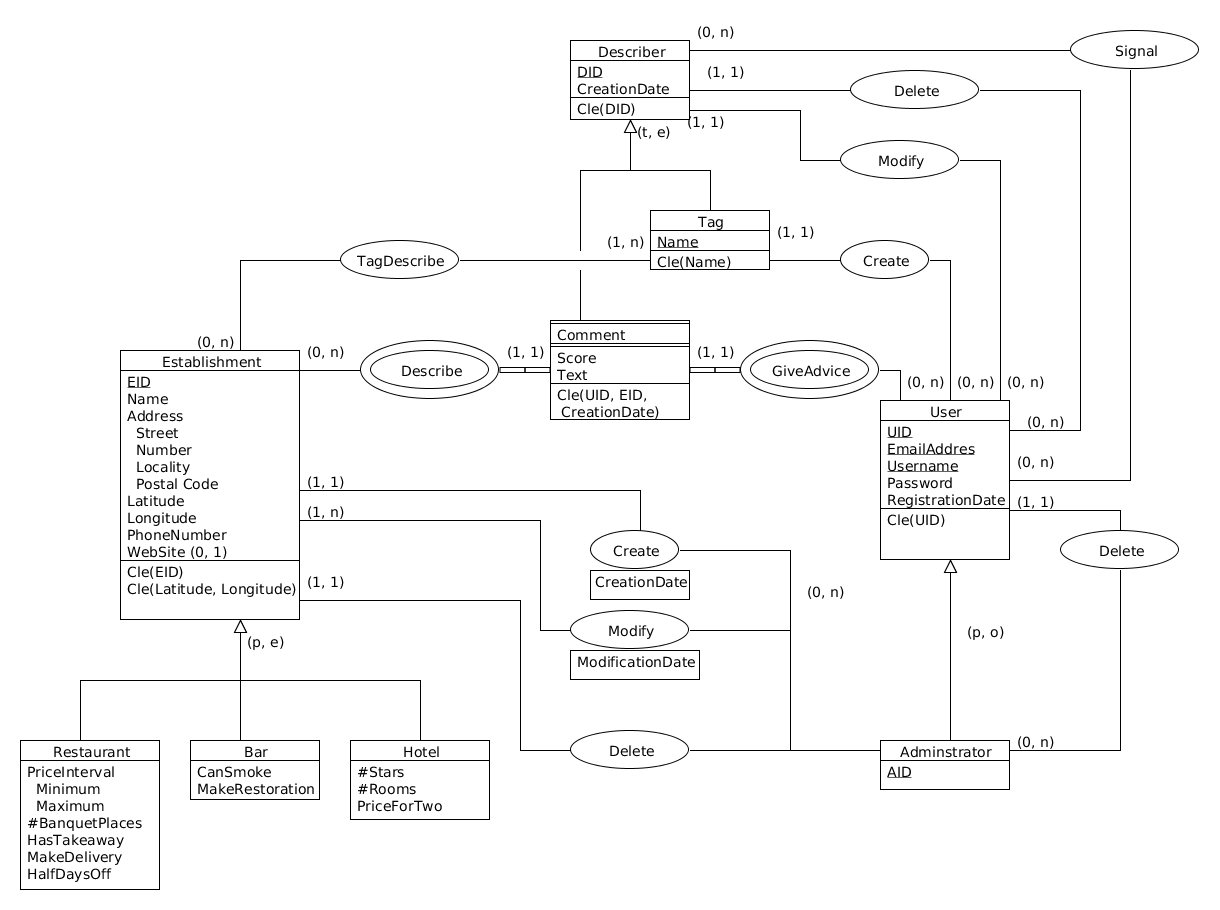
\includegraphics[scale=0.48]{model.png}}


\section*{Contraintes d'intégrité}

\begin{itemize}
    \item L'\textit{UID} Et L'\textit{EID}  sont respectivement  unique à chaque \textsl{User} et \textsl{Establishement}.
    
    \item \textit{User.EmailAdress} est unique.
    
    \item Le \textsl{User} doit impérativement être connecté pour pouvoir effectuer un \textsl{Comment}.
    
    \item \textsl{Comment.Score} varie entre 0 et 5.
    
    \item \textsl{Comment.Text} est fixé à maximum 200 caractères .
    
    \item La taille de \textit{User.Password} varie entre 4 et 16 caractères.
    
    \item Le \textsl{User} a le droit d'écrire un \textsl{Comment} par jour par \textsl{Establishement}.
    
    \item Le \textsl{User} ne peut apposer qu'une seule fois le même \textsl{Tag} sur un même \textsl{Establishement}.
    
    \item Un \textsl{User} a le droit de signaler un \textsl{Describer} d'un autre \textsl{User}, si celui-ci utilise un langage inadéquat ou si le commentaire porte des propos racistes ou injurieux.

    \item L' \textsl{Administrator} a la possibilité de supprimer un \textsl{User} si nécessaire.

    \item Tous les \textsl{Administrator} peuvent modifier ou supprimer n'importe quel \textsl{Establishment}.
    
    \item Le \textsl{User} ayant créer le \textsl{Describer} peut le modifier, ou le supprimer.
    
    \item Un \textsl{Administrator} peut uniquement supprimer les \textsl{Describer}, pas les modifier. Si il modifier un \textsl{Describer}, c'est uniquement ceux que lui même a créé.

\end{itemize}

\section*{Remarques}
    \begin{itemize}
        \item Pour les demi-jours de fermeture des \textsl{Restaurant}, nous avons choisi de stocker ces demi-jours en un tableau de \texttt{boolean}. Il est également possible d'utiliser une entité \textsl{DaysOff} qui sera en relation avec \textsl{Establishment}.
        \item Pour éviter que les établissements triche avec des utilisateurs robots, nous utiliserons un système \textsl{reCAPTCHA} pour les inscriptions des utilisateurs.
        
    \end{itemize}

\section*{Modèle relationnel}
\begin{itemize}
    
    \item Establishment(\underline{EID}, Name, Latitude, Longitude, PhoneNumber, Modified, \textsl{WebSite})

    \item Restaurant(\underline{EID}, PriceMinimum, PriceMaximum, BanquetPlaces, HasTakeaway, MakeDelivery, HalfDaysOff)

    \begin{itemize}
        \item Restaurant.EID reference Etablissment.EID.
    \end{itemize}

    \item Bar(\underline{EID}, CanSmoke, MakeRestoration)
    
    \begin{itemize}
        \item Bar.EID reference Etablissment.EID.
    \end{itemize}

    \item Hotel(\underline{EID}, NoStars, NoRooms, PriceForTwo)

    \begin{itemize}
        \item Hotel.EID reference Etablissment.EID.
    \end{itemize}

    \item Address(\underline{EID}, Street, No, Locality, PostalCode)

    \begin{itemize}
        \item Address.EID reference Etablissment.EID.
    \end{itemize}

    \item User(\underline{UID}, \underline{EmailAddress}, \underline{Username}, Password, RegistrationDate) 

    \item Administrator(\underline{UID}, \underline{AID}) 

    \begin{itemize}
        \item Administrator.UID fait référence a User.UID.
    \end{itemize}

    \item EstablishmentCreation(\underline{EID}, \underline{AID}, CreationDate)
    
    \begin{itemize}
        \item EstablishmentCreation.EID réference Establishment.EID.
        \item EstablishmentCreation.AID réference Administrator.AID.
    \end{itemize}
    
    \item EstablishmentModification(\underline{OldEID}, \underline{NewEID}, \underline{AID}, ModificationDate)

    \begin{itemize}
        \item EstablishmentModification.OldEID réference Establishment.EID.
        \item EstablishmentModification.NewEID réference Establishment.EID.
    \end{itemize}
    
    \item EstablishmentDeletion(\underline{EID}, \underline{AID}, DeletionDate)

    \begin{itemize}
        \item EstablishmentDeletion.EID réference Establishment.EID.
        \item EstablishmentDeletion.AID réference Administrator.AID.
    \end{itemize}
    
    \item UserDeletion(\underline{UID}, \underline{AID}, DeletionDate)
    
    \begin{itemize}
        \item UserDeletion.UID réference User.UID.
        \item UserDeletion.AID réference Administrator.AID.
    \end{itemize}

    
    \item DescriberDeletion(\underline{DID}, \underline{UID}, DeletionDate)

    \item DescriberModification(\underline{OldDID}, \underline{NewDID}, \underline{UID}, ModificationDate)
    
    \item Comment(\underline{DID}, \underline{UID, EID, CreationDate}, Score, Text, Modified) 

    \item Tag(\underline{DID}, \underline{Name}, \underline{UID}, CreationDate, Modified)

    \begin{itemize}
        \item Tag.UID réference User.UID.
    \end{itemize}

    \item Signal(\underline{DID}, \underline{SignalerUID})

    \item TagDescribe(\underline{Name}, \underline{EID}, \underline{UID})

    \begin{itemize}
        \item TagDescribe.Name réference Tag.Name.
        \item TagDescribe.EID réference Establishement.EID.
        \item TagDescribe.UID réference User.UID.
    \end{itemize}


\end{itemize}

\section*{Remarques}

\begin{itemize}
    \item Un \textsl{Establishment} ne peut pas existé sans qu'il soit associé a un \textsl{Restaurant}, \textsl{Bar} ou \textsl{Hotel}.
    
    \item un \textsl{User.UID} n'existant pas dans une \textsl{Administrator.UID} est un simple utilisateur n'ayant pas de droit de création/modification/suppression d'un établissement ou de suppression d'un \textsl{Describer} d'un autre \textsl{User} ou d'un \textsl{User}.
    
    \item La modification d'un \textsl{Establishment} étant possible, et que nous voulons garder les traces de modifications, il a été décidé que pour chaque modification un nouvelle \textsl{Establishment} sera créé. Pour savoir si un \textsl{Establishment} a été modifié il suffit de voir son champ \textsl{Establishment.Modified}. Si cette valeur est à \texttt{true}, c'est qu'il a été modifié et qu'il suffit donc de récuperer le nouvelle \textsl{Establishment.EID} via la relation \textsl{EstablishmentModification}. \textsl{Establishment.OldEID} référence l'\textsl{Establishment} ayant été modifié, et \textsl{Establishment.NewEID} référence l'\textsl{Establishment} où les modifications ont été apporté.

    \item Les \textsl{Describer} suivent le même principe de modification que les \textsl{Establishment}.

    \item \textsl{EstablishementModification.OldEID} et \textsl{EstablishmentModification.NewEID} ne peuvent pas être identique.
    
    \item \textsl{DescriberModification.OldDID} et \textsl{DescriberModification.NewDID} ne peuvent pas être identique.

    \item \textsl{UserDeletion.UID} ne peut pas référencer le {Administrator.UID} associé à \textsl{UserDeletion.AID}

    \item DID doit être unique entre les entités \textsl{Comment} et \textsl{Tag}.

\end{itemize}


\end{document}


